% !TEX program = xelatex
% Style học từ D:\AI_RTR\Realtime-Robotics\docs\slides\turn_7\slide.tex
% Nguyên tắc: ít chữ. Hình/bảng nói số; chữ chỉ nói NGHĨA, một câu ngắn.
\documentclass[aspectratio=169,10pt]{beamer}

\usetheme{metropolis}
\metroset{sectionpage=progressbar, numbering=fraction, block=fill, progressbar=frametitle}
\usefonttheme{professionalfonts}

\usepackage{fontspec}          % giữ XeLaTeX cho tiếng Việt
\setsansfont{Segoe UI}
\setmonofont{Consolas}
\usepackage{fvextra}
\usepackage{booktabs}
\usepackage{makecell}          % \makecell nhiều dòng trong ô
\usepackage{colortbl}          % \rowcolor
\usepackage{xcolor}
\graphicspath{{figs/}}

% ---- Màu ngữ nghĩa, mượn từ deck tham chiếu ----
\newcommand{\good}[1]{\textcolor{green!45!black}{\textbf{#1}}}   % kết quả chốt / khẳng định
\newcommand{\weak}[1]{\textcolor{red!70!black}{\textbf{#1}}}     % điểm yếu / thất bại
\definecolor{hirow}{HTML}{E4F1EC}                                % nền hàng punchline

% Câu chốt: MỘT dòng ngắn, xanh, canh đáy khung
\newcommand{\take}[1]{\vfill{\footnotesize\textcolor{green!45!black}{#1}}}

% Nhãn nguồn đáp án: đọc thẳng vs phải tự tính
\newcommand{\rd}{{\footnotesize\textcolor{green!45!black}{\textbf{[đọc]}}}}
\newcommand{\sm}{{\footnotesize\textcolor{orange!80!black}{\textbf{[tính]}}}}

\newcommand{\promptbox}[2]{\VerbatimInput[breaklines=true,breakanywhere=true,%
  breaksymbolleft={},breakautoindent=true,%
  fontsize=#1,baselinestretch=0.92,frame=single,framesep=4pt,%
  rulecolor=\color{black!35},formatcom=\color{black!85}]{#2}}

\title{Tác nhân LLM trong trò chơi rủi ro tập thể --- Turn 2}
\subtitle{Model lớn (scaling) \enspace\&\enspace Đọc-hiểu luật chơi (comprehension)}
\date{\today}
\author{Báo cáo nghiên cứu}

\begin{document}
\maketitle

% ======================================================================
\section{Turn này làm gì}

\begin{frame}{Nhắc lại: Turn trước ba model nhỏ chơi khác người}
  \begin{block}{Ba bất thường ở baseline}
    \begin{itemize}\setlength\itemsep{4pt}
      \item Phớt lờ rủi ro: 90/50/10\% $\to$ vẫn \good{$\sim$100\%} (người: 50$\to$10$\to$0\%)
      \item Hợp tác tăng dần về cuối --- ngược với người
      \item Đóng vượt mục tiêu: Qwen 233, Llama 185, Gemma 129 \;(/240)
    \end{itemize}
  \end{block}
  \begin{exampleblock}{Hai câu hỏi $\Rightarrow$ hai thí nghiệm Turn này}
    \begin{itemize}\setlength\itemsep{4pt}
      \item Do model \emph{nhỏ}? \quad$\to$\quad \alert{thử model lớn}
      \item Không hiểu luật, hay hiểu mà cố phớt lờ? \quad$\to$\quad \alert{kiểm tra đọc-hiểu}
    \end{itemize}
  \end{exampleblock}
\end{frame}

\begin{frame}{Hai thí nghiệm --- tổng quan}
  \centering
  \setlength{\tabcolsep}{10pt}\renewcommand{\arraystretch}{1.3}
  \begin{tabular}{lll}
    \toprule
    & \textbf{1 --- Model lớn} & \textbf{2 --- Đọc-hiểu} \\
    \midrule
    Trả lời   & do cỡ model? & có thật sự hiểu luật? \\
    Model     & \makecell[l]{Qwen 7B$\to$32B$\to$72B\\Gemma 9B$\to$27B, Llama 8B$\to$70B} & 3 nhỏ + 2 lớn (32B/27B) \\
    Setup     & baseline như Turn 1 & hỏi xen kẽ trong ván \\
    Đo        & tỉ lệ đạt, đóng góp, nhịp & đúng/sai 20 loại câu \\
    Quy mô    & 60 ván/model (7 model) & $\sim$54.500 câu/model \\
    \bottomrule
  \end{tabular}
  \take{Phần đọc-hiểu phỏng theo \emph{``Nicer Than Humans''} (Fontana et al.\ 2024).}
\end{frame}

% ======================================================================
\section{Mở rộng 1 --- Model lớn (scaling)}

\begin{frame}{Cách làm}
  \begin{block}{Thao tác}
    Giữ nguyên baseline Turn 1 --- chỉ \textbf{đổi model lớn}: Qwen 7B$\to$32B$\to$\textbf{72B}, Gemma 9B$\to$27B, và \textbf{Llama 8B$\to$70B} (đủ ba họ, mỗi họ một model lớn).
  \end{block}
  \begin{exampleblock}{Hai khả năng đối nghịch}
    \begin{itemize}\setlength\itemsep{4pt}
      \item Do model nhỏ \;$\to$\; model lớn sẽ biết ``sợ'' rủi ro
      \item Đặc tính chung \;$\to$\; vẫn phớt lờ, chỉ đổi cách tiêu tiền
    \end{itemize}
  \end{exampleblock}
\end{frame}

\begin{frame}{Model càng lớn, cả ba họ càng hội tụ về “vừa đủ”}
  \centering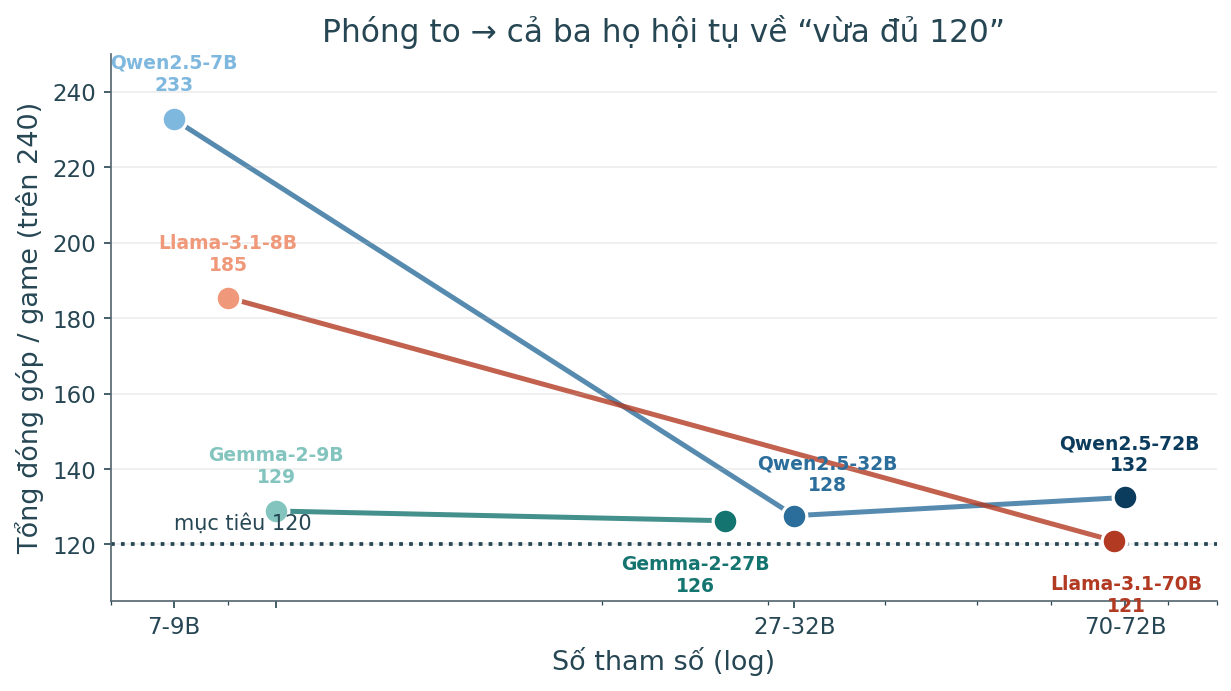
\includegraphics[height=0.68\textheight]{L1_scaling_contrib.png}
  \take{Qwen \weak{233}$\to$\good{128}$\to$132 (bão hoà); Llama \weak{185}$\to$\good{121}; Gemma đứng yên. Ba họ chụm về mốc 120.}
\end{frame}

\begin{frame}{Nhưng model lớn vẫn không biết sợ rủi ro}
  \centering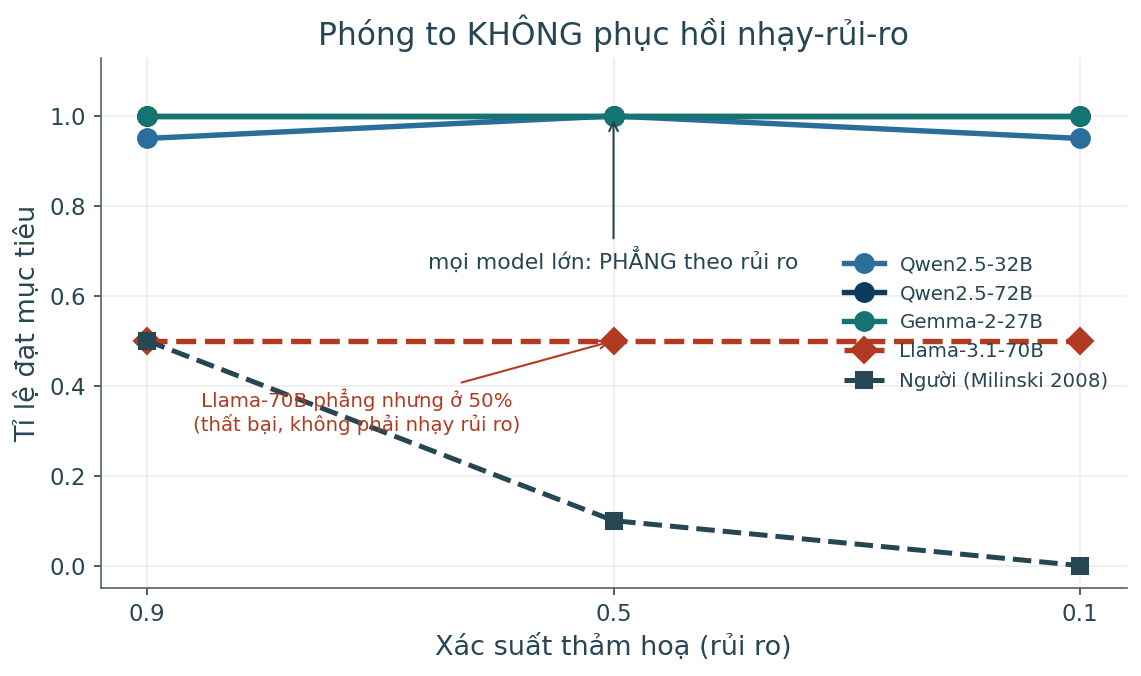
\includegraphics[height=0.68\textheight]{L2_scaling_reach.png}
  \take{Qwen-32B/72B \& Gemma-27B vẫn \good{$\sim$100\%} ở mọi mức rủi ro. Llama-70B \weak{phẳng ở 50\%} --- thất bại, \emph{không phải} nhạy rủi ro.}
\end{frame}

\begin{frame}{Model lớn đầu tiên THẤT BẠI --- nhưng do ngôn ngữ}
  \centering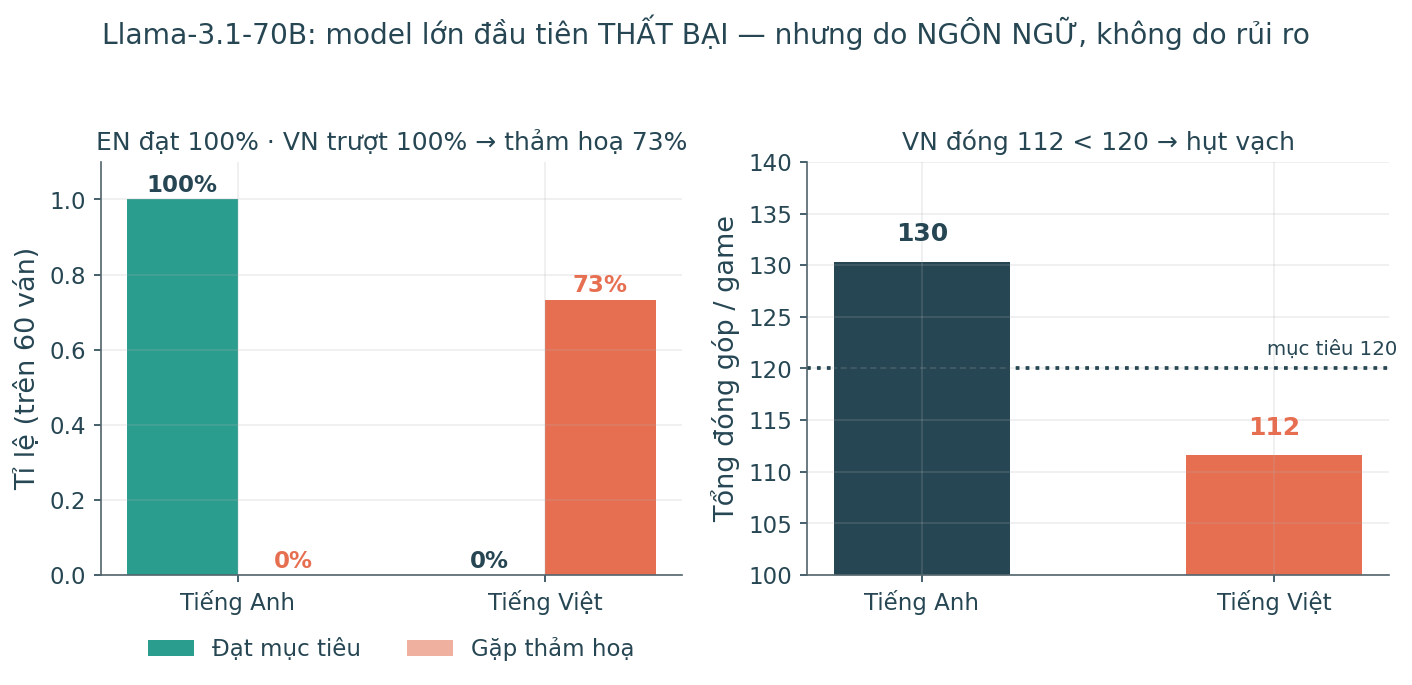
\includegraphics[height=0.62\textheight]{L6_llama70_lang_collapse.png}
  \take{Llama-70B: EN đạt \good{100\%}; VN đóng \weak{112$<$120} $\to$ trượt \weak{100\%}, thảm hoạ \weak{73\%}. Trục ngôn ngữ đủ mạnh để gây hậu quả thật.}
\end{frame}

\begin{frame}{Lớn lên, cả họ Qwen \& Llama bỏ thói quen đóng dư}
  \centering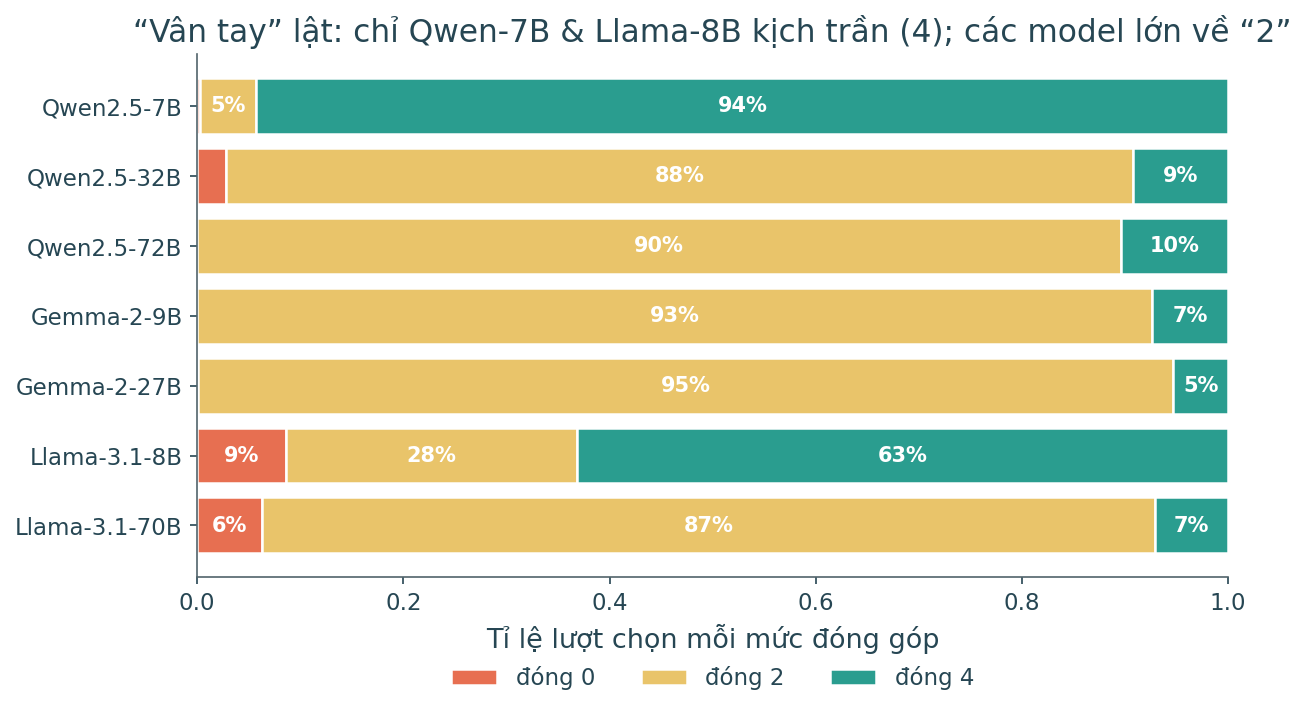
\includegraphics[height=0.66\textheight]{L3_choice_flip.png}
  \take{Chỉ Qwen-7B (\weak{94\% chọn 4}) \& Llama-8B (63\%) kịch trần. Mọi model lớn về \good{mức ``2''} như Gemma.}
\end{frame}

\begin{frame}{Vẫn đóng tăng dần --- riêng Llama-70B bỏ cuộc vòng chót}
  \centering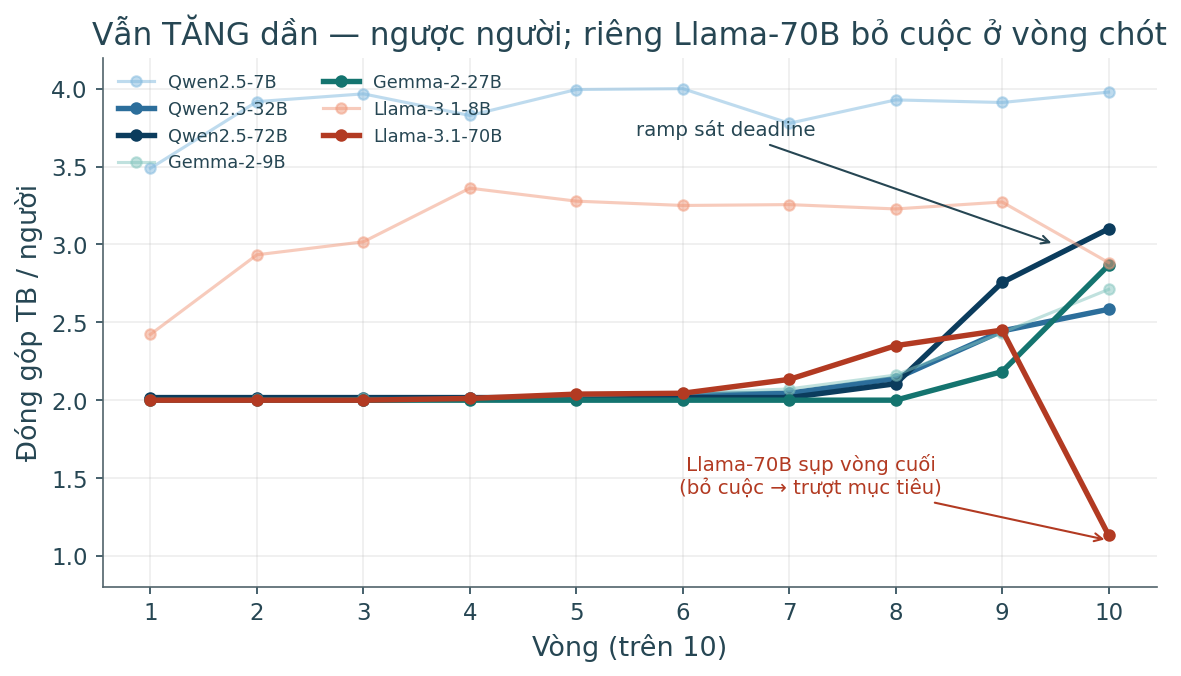
\includegraphics[height=0.66\textheight]{L4_scaling_dynamics.png}
  \take{Model lớn giữ mức 2 rồi vọt ở vòng 9--10 (vẫn \alert{tăng dần, ngược người}). Riêng Llama-70B \weak{sụp 2.5$\to$1.1} vòng cuối $\to$ trượt vạch.}
\end{frame}

\begin{frame}{Trục ngôn ngữ không mất khi phóng to}
  \centering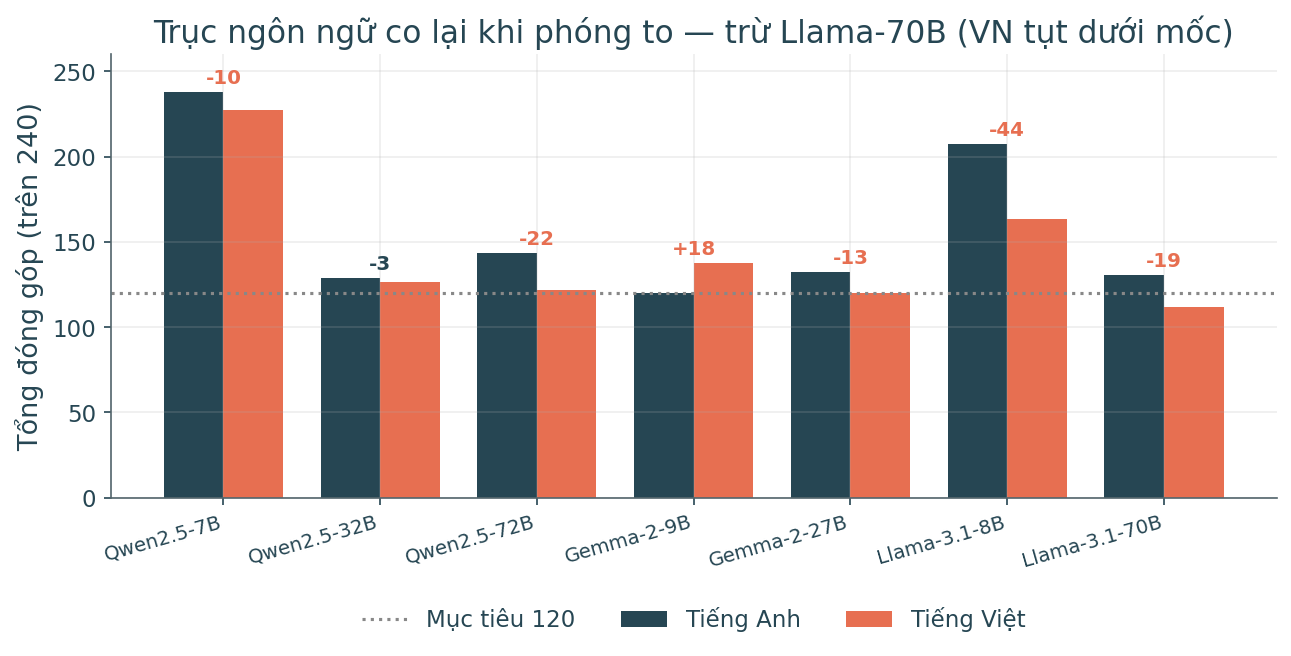
\includegraphics[height=0.64\textheight]{L5_scaling_lang.png}
  \take{Chênh Anh--Việt còn ở mọi cỡ ($-3$ đến $-22$). Điều mới: ở Llama-70B mức VN \weak{tụt dưới mốc 120} $\to$ hụt vạch, thảm hoạ.}
\end{frame}

\begin{frame}{Tóm lại về model lớn}
  \centering
  \setlength{\tabcolsep}{10pt}\renewcommand{\arraystretch}{1.3}
  \begin{tabular}{lll}
    \toprule
    Khía cạnh & Nhỏ (7--9B) & Lớn (27--72B) \\
    \midrule
    Phản ứng rủi ro   & Không & \alert{Vẫn không} \\
    Nhịp hợp tác      & Tăng dần & \alert{Vẫn tăng dần} \\
    \rowcolor{hirow} Đóng góp Qwen (7$\to$32$\to$72B) & \weak{233} & \good{128 $\to$ 132} \\
    Đóng góp Llama (8$\to$70B) & 185 & \good{121} \\
    Đóng góp Gemma (9$\to$27B) & 129 & 126 \\
    \rowcolor{hirow} Tỉ lệ đạt mục tiêu & 100\% & \makecell[l]{$\sim$100\% \emph{trừ} Llama-70B\\(\weak{50\%}, VN thất bại)} \\
    \bottomrule
  \end{tabular}
  \take{Model lớn \emph{tiêu tiền khôn hơn}, KHÔNG \emph{biết sợ rủi ro hơn}. Llama-70B lộ điểm gãy \alert{ngôn ngữ}.}
\end{frame}

% ======================================================================
\section{Mở rộng 2 --- Kiểm tra đọc-hiểu}

\begin{frame}{Đo đọc-hiểu bằng cách nào?}
  \begin{block}{Hỏi --- xen kẽ trong lúc chơi (in-situ)}
    Mỗi vòng hỏi thêm về chính ván đó, qua lượt \emph{riêng} $\Rightarrow$ \textbf{không đổi nước đi} (đã kiểm chứng).
  \end{block}
  \begin{block}{Chấm --- so đáp án engine}
    Ground-truth tính sẵn, đúng/sai tự động. \textbf{$\sim$54.500 câu/model}; nay đo cả \textbf{2 model lớn} (Qwen-32B, Gemma-27B) để xem scaling có ``chữa'' được không.
  \end{block}
  \begin{exampleblock}{Ba nhóm câu}
    \textbf{Rules} đọc luật \quad$\bullet$\quad \textbf{Time} tra lịch sử \quad$\bullet$\quad \textbf{State} cộng dồn
  \end{exampleblock}
\end{frame}

\begin{frame}{Bộ câu hỏi thật --- 20 câu / lượt}
  {\footnotesize \rd{} = in sẵn trong prompt, chỉ đọc \quad$\vert$\quad \sm{} = phải tự tính từ lịch sử}
  \smallskip
  \begin{columns}[T]
    \begin{column}{0.49\textwidth}
      {\scriptsize\color{green!45!black}\textbf{RULES} --- 8 câu (toàn \rd)}\par
      {\scriptsize
      \begin{enumerate}\setlength\itemsep{0.5pt}
        \item Mỗi vòng đóng những mức nào? \;(0/2/4)
        \item Vốn ban đầu mỗi người? \;(40)
        \item Mục tiêu chung cả game? \;(120)
        \item Game dài mấy vòng? \;(10)
        \item Trượt mục tiêu, \% mất hết? \;(90/50/10)
        \item Trượt mà gặp thảm hoạ, còn bao nhiêu? \;(0)
        \item Mức đóng tối đa một vòng? \;(4)
        \item Mức đóng tối thiểu một vòng? \;(0)
      \end{enumerate}}
      \smallskip
      {\scriptsize\color{green!45!black}\textbf{TIME} --- 4 câu (tra lịch sử)}\par
      {\scriptsize
      \begin{enumerate}\setlength\itemsep{0.5pt}\setcounter{enumi}{8}
        \item Đang ở vòng thứ mấy? \rd
        \item Vòng $i$, ghế P$x$ đóng bao nhiêu? \rd
        \item Vòng $i$, chính bạn đóng bao nhiêu? \rd
        \item Vòng $i$, cả 6 người đóng tổng? \sm
      \end{enumerate}}
    \end{column}
    \begin{column}{0.49\textwidth}
      {\scriptsize\color{green!45!black}\textbf{STATE} --- 8 câu (tích luỹ)}\par
      {\scriptsize
      \begin{enumerate}\setlength\itemsep{0.5pt}\setcounter{enumi}{12}
        \item Tổng quỹ chung đến giờ? \sm
        \item Còn thiếu bao nhiêu để đạt 120? \sm
        \item Ghế P$x$ đã đóng tổng cộng? \sm
        \item Chính bạn đã đóng tổng cộng? \sm
        \item Bạn còn lại bao nhiêu vốn? \rd
        \item Ghế P$x$ đóng đúng mức 4 mấy lần? \sm
        \item Còn mấy vòng nữa (kể cả vòng này)? \sm
        \item Nhóm đã đạt mục tiêu chưa? \sm
      \end{enumerate}}
      \smallskip
      \begin{block}{Ý đồ}
        {\scriptsize Rules/Time = \emph{đọc}; State = \emph{cộng dồn}. Tách ra để biết yếu ở \emph{hiểu luật} hay \emph{tính trạng thái}.}
      \end{block}
    \end{column}
  \end{columns}
\end{frame}

\begin{frame}{Độ chính xác từng câu --- 20 câu, ba model}
  \centering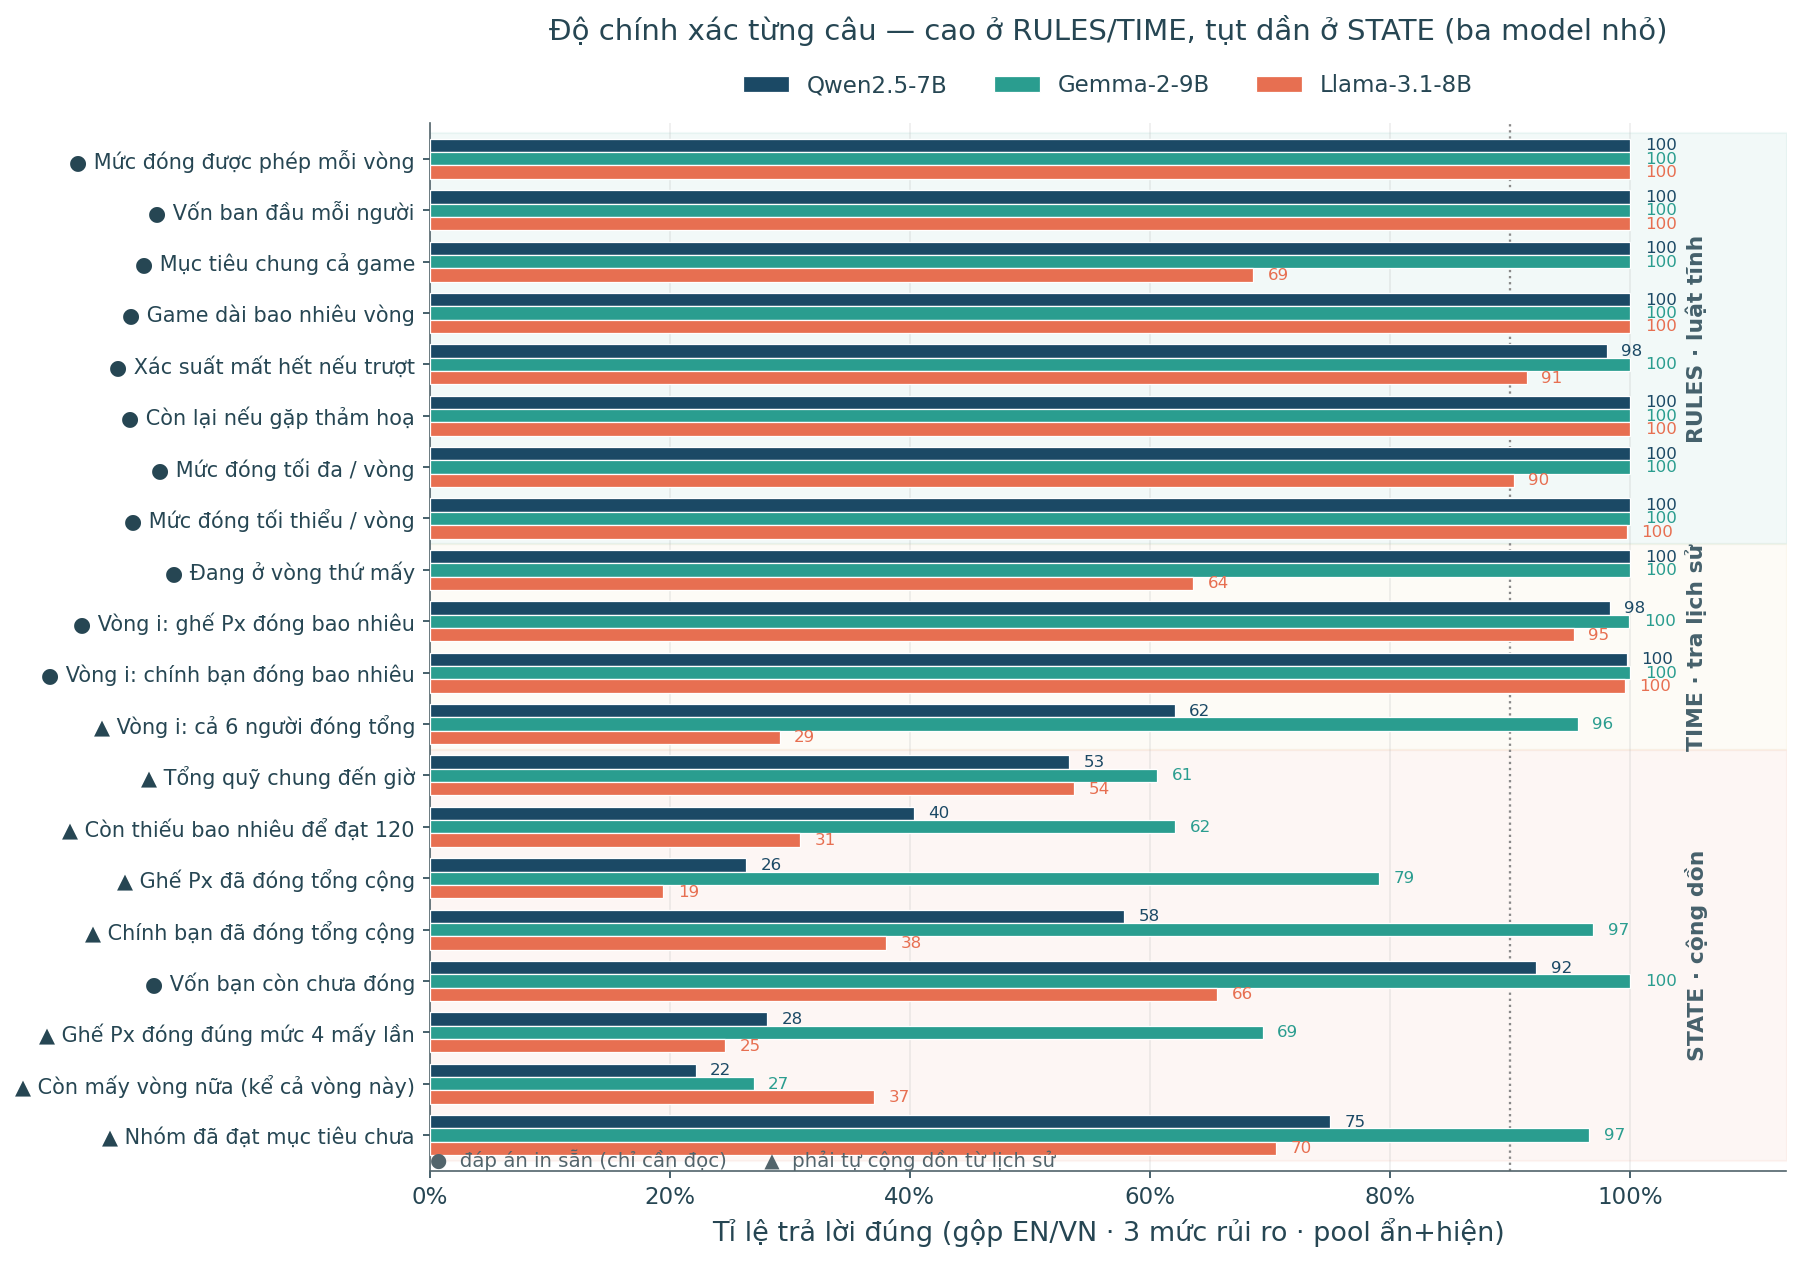
\includegraphics[height=0.9\textheight]{K0_comp_per_question.png}
\end{frame}

\begin{frame}[fragile]{Một probe hoàn chỉnh}
  \promptbox{\fontsize{6}{6.6}\selectfont}{assets/probe_prompt_full.txt}
  \take{Prompt in sẵn \emph{remaining money: 34} nhưng \alert{KHÔNG in tổng quỹ} $\Rightarrow$ phải tự cộng 12+12+12.}
\end{frame}

\begin{frame}[fragile]{Trả lời thật --- biết luật, nhưng không cộng được}
  \promptbox{\fontsize{7.4}{8.6}\selectfont}{assets/probe_examples.txt}
  \take{Pool ẩn: model trả \weak{24} (một vòng) thay vì 96. In sẵn tổng: \good{đúng} ngay. Biết \% rủi ro (90).}
\end{frame}

\begin{frame}{Model lớn cộng dồn tốt hơn hẳn --- nhưng chưa kín}
  \centering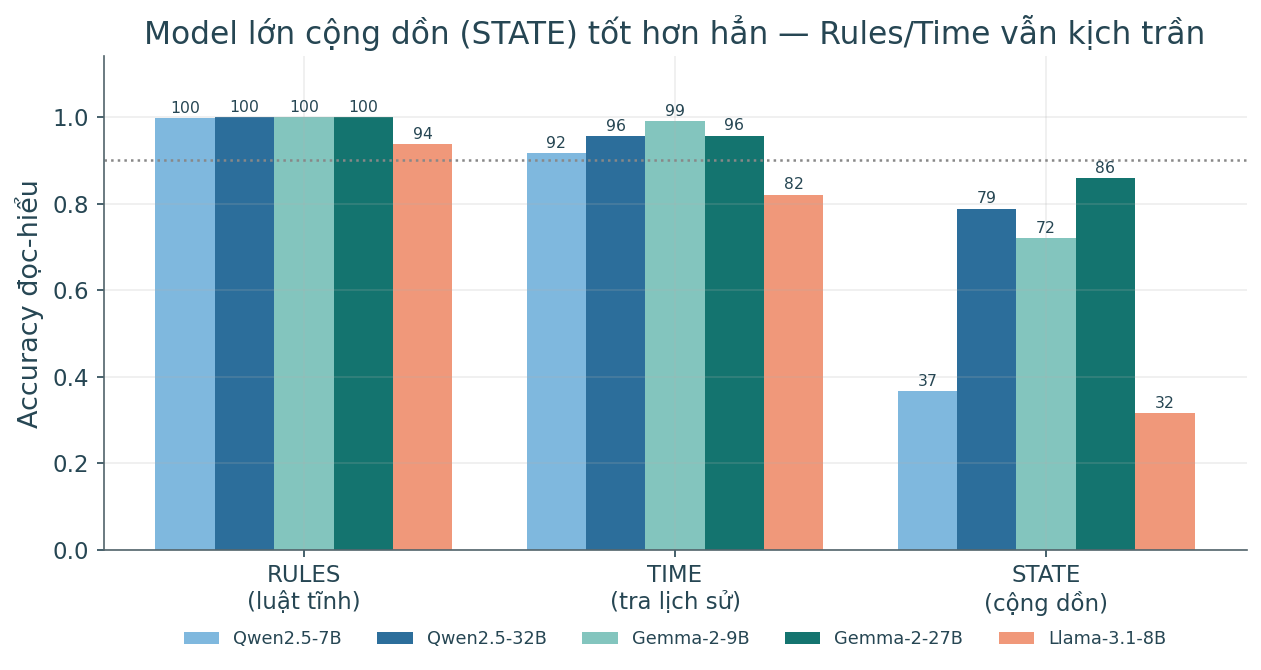
\includegraphics[height=0.64\textheight]{K1_comp_category.png}
  \take{Rules/Time đã kịch trần ở mọi cỡ. Scaling nâng riêng State: Qwen \weak{37}$\to$\good{79}, Gemma \weak{72}$\to$\good{86}. Lỗ hổng là \emph{số học}, không phải luật.}
\end{frame}

\begin{frame}{Kết quả sắc nhất: đọc được $\neq$ cộng được}
  \centering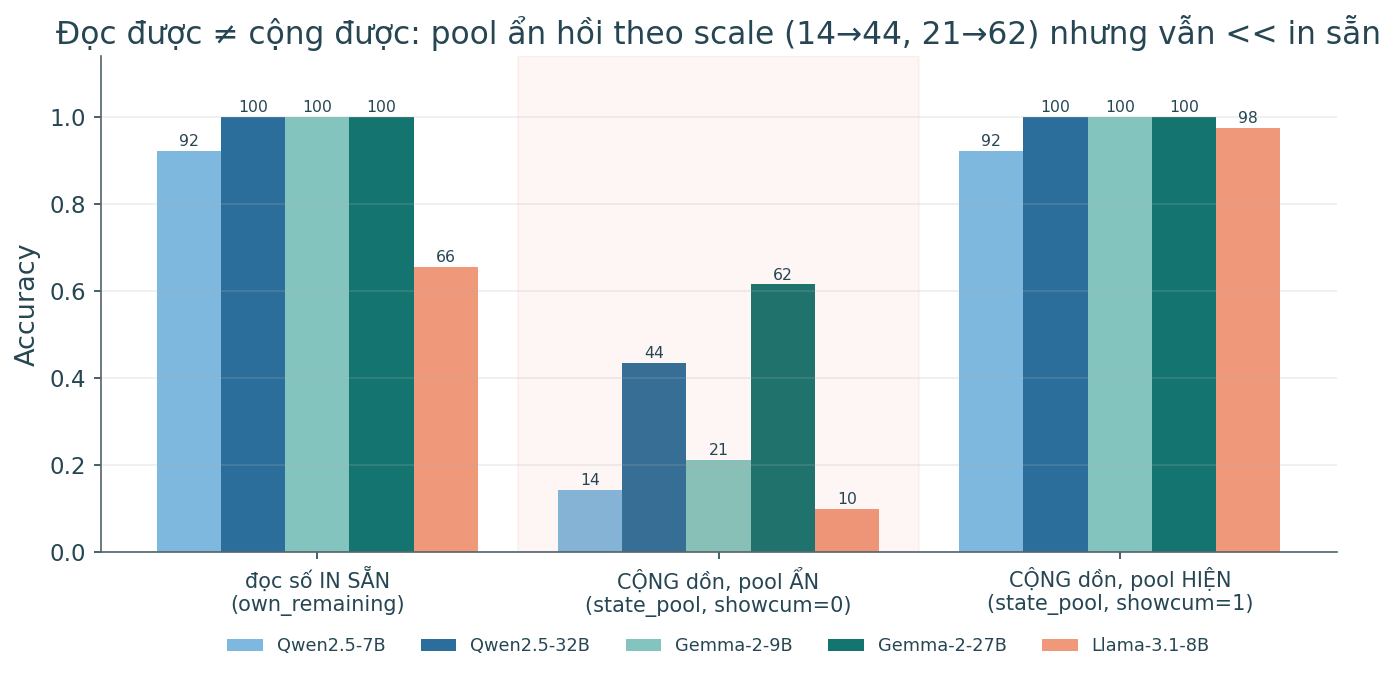
\includegraphics[height=0.62\textheight]{K2_comp_read_vs_add.png}
  \take{Pool ẩn (phải tự cộng) hồi theo scale: Qwen \weak{14}$\to$44, Gemma \weak{21}$\to$\good{62}; nhưng in sẵn tổng là \good{$\sim$100\%}. Khoảng cách co lại, chưa mất.}
\end{frame}

\begin{frame}{Phép thử then chốt: model BIẾT rủi ro, chỉ phớt lờ}
  \centering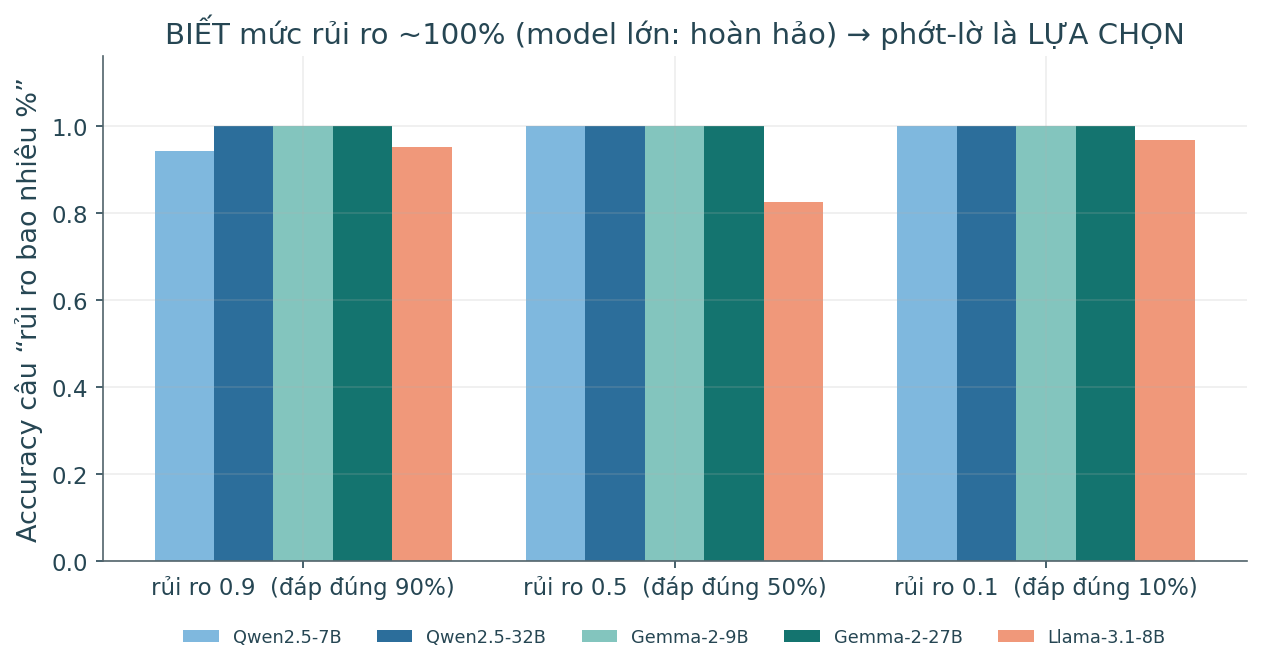
\includegraphics[height=0.60\textheight]{K3_comp_risk_gate.png}
  \take{Câu ``\% rủi ro'' đúng \good{$\sim$100\%} --- model lớn \good{hoàn hảo mọi mức}. Phớt lờ rủi ro KHÔNG do hiểu sai; biết mà vẫn chọn như nhau.}
\end{frame}

\begin{frame}{Tiếng Việt làm yếu đúng khâu cộng dồn}
  \centering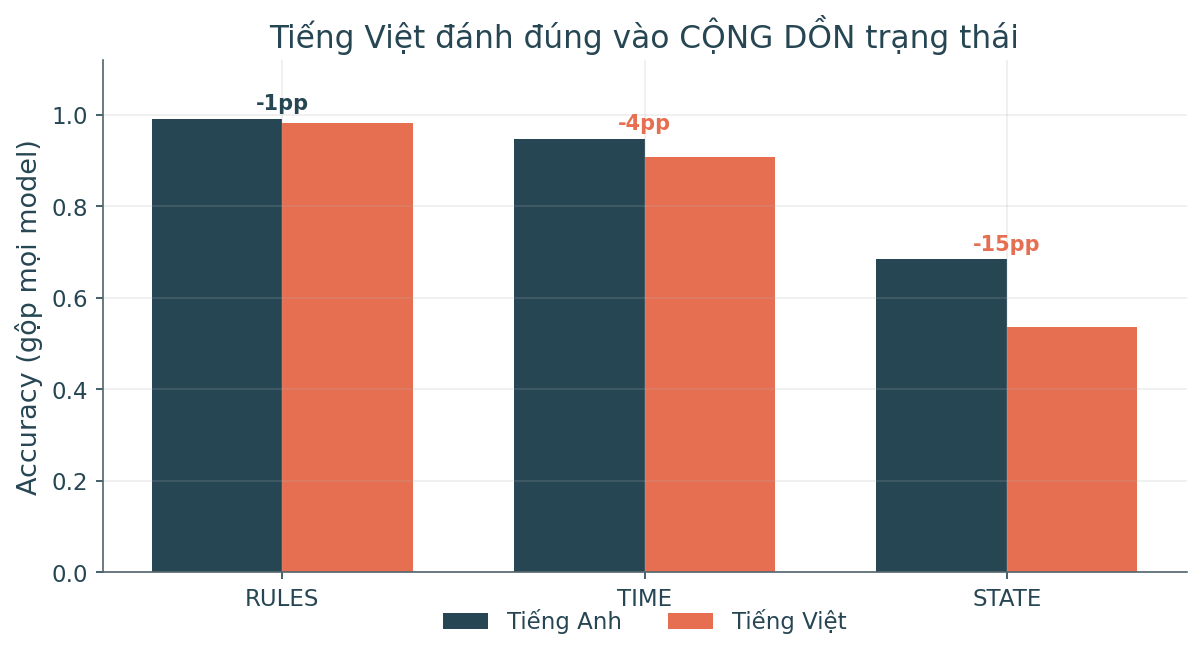
\includegraphics[height=0.60\textheight]{K4_comp_lang.png}
  \take{Rules/Time gần như không đổi ($-1$, $-4$đ\%); State rớt \weak{$-15$đ\%} ở tiếng Việt (gộp cả model lớn). Ngôn ngữ đánh đúng khâu yếu nhất.}
\end{frame}

\begin{frame}{Bảng chi tiết 20 loại câu (phụ lục)}
  \centering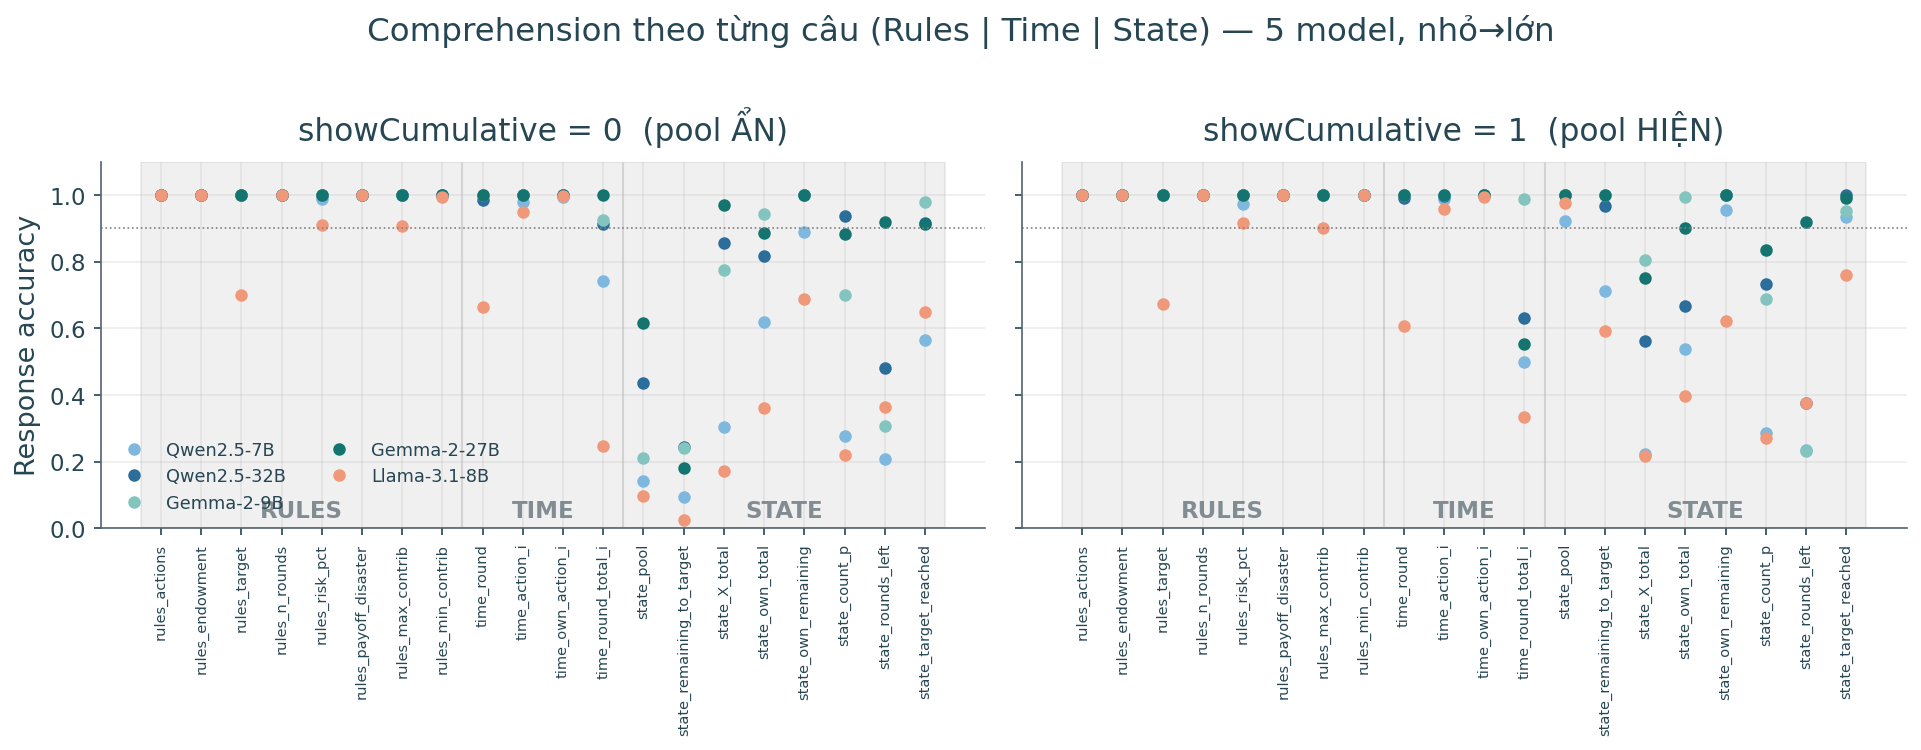
\includegraphics[height=0.66\textheight]{K5_comp_figure1.png}
  \take{Năm model, nhỏ$\to$lớn: Rules kịch trần; Time tốt trừ ``tổng 6 người/vòng''; State cộng dồn cải thiện theo cỡ nhưng vẫn thấp nhất.}
\end{frame}

% ======================================================================
\section{Tổng kết Turn 2}

\begin{frame}{Hai mảnh ghép vào bức tranh chung}
  \begin{block}{Hợp tác của LLM là \emph{thói quen}, không phải \emph{tính toán}}
    \begin{itemize}\setlength\itemsep{3pt}
      \item Hiểu luật + biết rủi ro (\good{$\sim$100\%}); cộng-dồn trạng thái yếu và \emph{chỉ hồi một phần} khi phóng to (pool ẩn 21$\to$\good{62\%})
      \item $\Rightarrow$ hợp tác là thiên hướng có sẵn, không phải suy luận theo trạng thái
      \item Scaling chỉ cắt phần đóng dư (233$\to$128): tiêu khôn hơn, vẫn phớt lờ rủi ro tới 72B
      \item Llama-70B: model lớn đầu tiên \weak{thất bại thật} --- nhưng do \alert{ngôn ngữ} (VN hụt vạch), không do rủi ro
    \end{itemize}
  \end{block}
  \take{Phớt lờ rủi ro: không do \emph{hiểu sai}, không do \emph{model nhỏ} $\Rightarrow$ \alert{thiên hướng hành vi} của lớp model này.}
\end{frame}

\begin{frame}{So với Turn trước}
  \centering
  \setlength{\tabcolsep}{11pt}\renewcommand{\arraystretch}{1.35}
  \begin{tabular}{lll}
    \toprule
    Câu hỏi & Turn trước & Turn này \\
    \midrule
    Do model nhỏ?        & giả thuyết & \weak{Không} --- 27/32B vẫn phẳng \\
    Hiểu luật?           & chưa đo    & \good{Có} --- Rules 94--100\% \\
    Biết mức rủi ro?     & chưa đo    & \good{Có} --- câu rủi ro $\sim$100\% \\
    Vì sao theo dõi quỹ sai? & ``thói quen'' & \weak{Không cộng dồn được} (10--21\%) \\
    Trục ngôn ngữ?       & đóng góp (Llama) & + \alert{số học} (State $-19$đ\% VN) \\
    \bottomrule
  \end{tabular}
  \take{Turn này \emph{khẳng định} \& \emph{giải thích} các bất thường Turn 1, không lật ngược.}
\end{frame}

\begin{frame}{Điểm thảo luận với thầy}
  \textbf{Scaling}
  \begin{itemize}\setlength\itemsep{2pt}
    \item Cần chạy Llama lớn (70B) để đủ cặp họ thứ ba không ạ?
    \item Qwen-32B tụt nhẹ tỉ lệ đạt (97\%) vì chơi sát vạch --- lấy \emph{đóng góp} làm biến chính?
  \end{itemize}
  \smallskip
  \textbf{Đọc-hiểu}
  \begin{itemize}\setlength\itemsep{2pt}
    \item ``Không cộng dồn'' là giới hạn số học hay do prompt quá dài? $\to$ thử cắt ngắn lịch sử.
    \item Đưa \emph{tổng quỹ in sẵn} vào prompt quyết định --- hợp tác có đổi khi được ``nhắc''?
  \end{itemize}
\end{frame}

\begin{frame}[standout]
  Model lớn: \textbf{tiêu tiền khôn hơn}, không \textbf{biết sợ rủi ro hơn}. \\[3mm]
  LLM \textbf{hiểu luật} \& \textbf{biết rủi ro}, nhưng \textbf{không cộng được trạng thái} --- \\
  hợp tác là \textbf{thói quen}, không phải tính toán.
\end{frame}

\end{document}
